\documentclass[12pt, a4paper]{article}

\usepackage[utf8]{inputenc}
\usepackage{graphicx} % to embed images
\usepackage{hyperref} % to link the table of contents
\usepackage{subcaption} %complex images
\usepackage{placeins} %floating
%\usepackage{pdflscape} %to allow single pages in landscape mode
\usepackage[top=1.25in, bottom=1.25in, left=1in, right=1in]{geometry}
\usepackage{verbatim} % include raw text file (for Alloy)
\usepackage[export]{adjustbox}

\title{Requirement Analysis and Specification Document}
\date{2017-10-26}
\author{
	Leonardo Bisica
	\and
	Alessandro Castellani
	\and
	Michele Cataldo
}

\begin{document}
	%%% titlepage %%%
	\begin{titlepage}
		\centering
		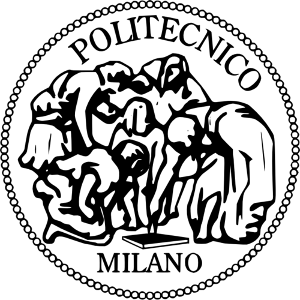
\includegraphics[width=5cm]{img/polimi_logo.png} % also works with logo.pdf
		\vfill
		{\bfseries\Large
			Travlendar+\\
			Requirement Analysis and Specification Document
			Version 0.1\\
			\vskip4cm
			Leonardo Bisica\\
			Alessandro Castellani\\
			Michele Cataldo\\
		}
		\vfill
		\vfill
	\end{titlepage}

	%%% table of contents %%%
	\tableofcontents
	\newpage

	%%% introduction %%%
	\section{Introduction}
		\subsection{Purpose}
		The document that you are reading is the \textit{Requirement Analysis and Specification Document} (RASD) for information system \textit{Travelandar+}.
		This start-up aims to help users in their everyday-life between appointment’s organization and transportation. No previous version about this application have been developed. 
We will start from describe Stakeholders’ aims (\textit{Goals} Section), from which we obtain, subsequently, functional and nonfunctional requirements (\textit{Requirements} Section) useful to describe the system.
		In addition we will need other 2 sections to have a complete overview of the model: \textit{Constraints} Section that describes constraints about the system and \textit{Domain Properties} Section that underlines limits of the software imposed by the world.
		After spoke about this first chapter we could analyze some scenarios and use case of the application.
			
		\subsection{Actual system}
			da fare
		
		\subsection{Scope}
		The aim of this project is to develop \textit{Travlendar+}, a calendar based mobile application.
Main functionality of the system is helping people in scheduling their meetings, by giving them useful information like traffic informations, public transportation and weather.
	Meetings could be scheduled through the entire region of Lombardy (Italy), and the main Italian cities connected via railway system, and could be several type of work meetings and personal meetings.
Furthermore the system can help the user by buying via mobile application public transportation tickets, or by reserving a car or a bike of a Sharing system, if it’s available in the current city.
In case of bad weather the system should find alternative moving solutions in order to replace walking path.
Naturally, the system must also allow the registration of new users; for the registration the system requests both personal and payment information. After registration, the user could immediately start scheduling his meetings.
			
		%TODO	
		\subsection{Goals}
		\begin{enumerate}
	\item
		[G1] System allows guest user to register with an username ad and a password; to complete the procedure user should confirm by 

	\item
		[G2] System Login

	\item 
		[G3] Registered User can create meetings 
	\item 
		[G4] Registered User can edit meetings
	\item 
		[G5] The application can automatically compute a personalized selection of travel times between appointments to choose from
	\item
		[G6] User can choose a preferred solution among the best ones
	\item
		[G7] The application warns the user if locations are unreachable in the allotted time
	\item
		[G8] Allow users to put constraints on different travel means and limit carbon footprints
	\item
		[G9] The application features additional user’s privileged time spans
	\item
		[G10] The application allows to arrange the trips : tickets for public services
	\item	
		[G11] The application allows the nearest shared vehicle to be found
	\item
		[G12] The application can obtain the position of the device and consequently of its user
		
\end{enumerate}	


		%TODO	
		\subsection{Domain properties}
		\input{Subsections/domain_properties.tex}
		%TODO	
		\subsection{Glossary}
		%\begin{description}
				\item[User] 
				\begin{itemize}
					\item First name;
					\item Last name; 
					\item Email;
					\item Username;
					\item Password;
					\item Payment information; this in particular includes:
						\begin{itemize}
							\item Credit card owner;
							\item Credit card number;
							\item Credit card expiration date;
							\item CVV number.
						\end{itemize}
				\end{itemize}
				
				\item[Guest] We name 'guests' all the people who are using the interface of the system without being registered or logged in. Guests can't access any functionality of \textit{Travlendar+} except for the registration process and the log in. 
				\item[Operative Zone] We name Operative Zone the area within we can place the location of an event. For the time being the Operative Zone coincide with all the cities and places within italian peninsula that can be reached by simply consulting the Google APIs. Naturally, such an area may be expanded in the future.
				\item[Influence Zone] We name Influence Zone the area within whose borders the mobile application can not only give travel time by car and on foot (the minimum standard given to us by Google APIs) but also where Travlendar+ can rely at least on a single car and bike sharing service. For starting, the Influence Zone will coincide with the city of Milan.
				\item
				\item[Registered User] A registered User is a former guest who inserted his/her own credentials in the system. After previous login, a Registered User can then create events, work on the timetable and ultimately is the end-user of Travlendar+.
				\item[Timetable]
				\item[Vehicle Sharing services/systems and a Shared Vehicle] By vehicle sharing we do not inted referring to a generic 'car-pooling' service. The usage of a shared vehicle may be either one of two types, car or bike sharing. A vehicle within the system operates only within the boundaries and parking zones imposed by its service; it can be picked up by any user registered to its corresponding system, used for the required amount of time (even though a maximum time is always fixed) and then parked in an allowed zone, ready to be picked by up again by another user. Eahc sharing system possesses an individual API			
				\item[Mobile Application] By mobile application we refer to a program conceived for Android and iOS operative systems, based on touch interfaces and able to run on portable devices. The logic of the mobile application is the system.
				\item[Appointment] An appointment is an event well delimited both in time and space, requiring the presence and the direct investment, in our case, of the user who creates it. Appointments fall in two categories : work appointments (that are often referred also as meetings) and personal appointments (the broader set encapsulating all other kinds of appointments, mainly regarding personal and family life)
				\item[Warning] A warning is a notification given by Travlendar+ mobile application to the operating System it is hosted by. It behaves as a standard system notification.
				\item[Travel Logic] By travel logic we refer to the logic that processes the distances and the transportation time within our operative and influcence zones. In the case at hand, in this first implementation, we're going to adopt as Travel Logic the Google Maps APIs.
\end{description}

		%TODO	
		\subsection{Assumptions}
		\subsection{Assumptions, dependencies, constraints}

	We've already given a formal and methodical definition of our problem, yet there are still some ambiguities which still need to be addresed.


		\begin{enumerate}
		
			\item Users do not create events outside the “operative zone”

			\item The devices Travlendar+ is installed on possess a well-functioning GPS for geo-localization

			\item If a registered User is willing to use the vehicle of a sharing network, we assume him to have downloaded the corresponding sharing-network app

			\item There’s no kind of dependency among the users of our system

			\item Any information coming from sharing services regarding position, rental, and payment won’t be double-checked by our system

			\item Information coming from external payment sites won’t be double checked by our system

			\item Buying public transportation tickets rely on the aforementioned external payment procedures

			\item System assumes the season passes submitted by the user only aid for filtering results and are not checked nor have any legal value

			\item System assumes that any car rental request is made by a person who’s allowed to make one. Only sharing services check the validity of documents; in addition to that we always assume the driver is the user who requests the rental

			\item The application doesn't act as a navigator, and isn't capable of giving live informations about the travel besides the ones that can arrive through notifications
			
		\end{enumerate}

			
			


		



		\subsection{Constrains}			
		%\input{Subsections/constrains.tex}

		\subsection{Identifying stakeholders}


	\newpage
	\section{Actors identifying}
	%\input{Subsections/actors}
	\newpage
	\section{Requirements}
	%
\subsection{Functional Requirements}

We now adopt a goal-based approach to determine the requirements associated with each one of the goals we have elaborated in Chapter 1.\\
We'll start numbering and exploring the goals we submitted.

\begin{itemize}

            \item \textit{[G1]} System allows guest user to register with an username ad and a password; to complete the procedure user should confirm by 
               
                  \begin{itemize}
                        \item [R.1.1] System should let registering user choose an username and password
                        \item [R.1.2] Every username corresponds to a single user
                        \item [R.1.3] Duplicate usernames aren’t allowed
                        \item [R.1.4] Registering user can't be already registered
                        \item [R.1.5] An unregistered user is locked out the application and can only see registration page
                        \item [R.1.6] User has to confirm by mail his registration
                  \end{itemize}
             
\item \textit{[G2]} System Login

                  \begin{itemize}
                        \item [R.2.1] User must be already registered to perform correct login
                        \item [R.2.2] User must remember username and password
                        \item [R.2.3] Only a correct combination of username and password will grant access
                        \item [R.2.4] Application will implement a password retrieval mechanism
                  \end{itemize}
                  
\item \textit{[G3]} Registered User can create appointments 

 \begin{itemize}
                        \item [R.3.1] User has to be registered and logged in the system in order to create an
appointment
                        \item [R.3.2] Appointments can be divided into work appointments (or meetings) and personal appointments
                        \item [R.3.3] Appointments require a location and a starting time and an end time
                        \item [R.3.4] Appointments location must be within the boundaries of the operative zone
                        \item [R.3.5] The chosen location can be within the boundaries of the influence zone
                        \item [R.3.5] There cannot be appointments with the same name, location and time
                        \item [R.3.6] Based on already existing appointments, system checks suitability of created new entries
                        \item [R.3.7] Appointment start time can't precede the actual system time at the moment of inserting it                        
                  \end{itemize}
                  
\item \textit{[G4]} Registered Users can edit meetings

                  \begin{itemize}
                       \item  [R.4.1] A modified meeting must respect all the constraint imposed during the creation of a new meeting, as in [G3]
                       \item [R.4.2] A meeting can be modified up until its end time
                       \item [R.4.3] If the location of the meeting is modified it gets 
                       \item [R.4.4] If the location of the meeting is modified system behaves as if such an event was inserted for the first time, calculating all possibile conflicts with pre-existing events
                       \item [R.5.5] No limit actually exists on the amount of times an event can be modified
                       \item [R.5.6] 
                     


                  \end{itemize}

\item \textit{[G5]} The application can automatically compute a personalized selection of travel times between appointments to choose from

                  \begin{itemize}
                        \item [R.5.1] System verifies the travel mean is feasible for the submitted appointments
                        \item [R.5.2] According to the type of appointment, the system submits the data to corresponding external services
                        \item [R.5.3] Based on meeting type and time of day system ranks all the solutions
                        \item [R.5.4] Time is calculated by imposing a start position submitted by the user as specificied in [G12]
                  \end{itemize}
                  
\item \textit{[G6]} User can choose a preferred solution among the best ones 

                   \begin{itemize}
                        \item [R.6.1] User must be able to choose between ranked solutions
                        \item [R.6.2] The application arranges a navigable view of feasible solutions
                        \item [R.6.3] 
                  \end{itemize}
                  
\item \textit{[G7]} The application warns the user if locations are unreachable in the allotted time 

\item \textit{[G8]} Allow users to put constraints on different travel means and limit carbon footprints

\item \textit{[G9]} The application features additional user’s privileged time spans 

\item \textit{[G10]} The application allows to arrange the trips : tickets for public services

\item \textit{[G11]} The application allows the nearest shared vehicle to be found and reserved

                   \begin{itemize}
                        \item [R.11.1] A shared vehicle belongs to a bike-sharing service or a car-sharing service
                        \item [R.12.2] All services linked to shared vehicles are automatically disabled if the location of a meeting out of the boundaries of the influence zone
                        \item [R.12.3] All sharing services have their own API and they must be referenced by our mobile application
                        \item [R.12.4] To find or reserve a vehicle it is required by our system the access to the external API of the required service
                        \item [R.12.5] To find or reserve a vehicle it's required that the user logins into the external corresponding service
                        \item [R.12.6] The external service can communicate with our mobile application. In case of reservation Travlendar+ checks if the mobile app corresponding to the desired services is installed on the system. All the following steps take place within such an environment, until control is returned to Travlendar+
                        \item [R.12.7] The location of all the vehicles are shown in the same view, merging data from different APIs
                        \item [R.12.8] The renting happens 
                        
                        
                    \end{itemize}

\item \textit{[G12]} The application can obtain the position of the device and consequently of its user
                   
                  \begin{itemize}
                        \item [R.12.1] User can manually insert a location
                        \item [R.12.2] The mobile device can track its current position through geo-localization
                        \item [R.12.3] Position of out the operative zone won't be accepted by the system
                   \end{itemize}


\item \textit{[G13]} EVENTUAL NAVIGATION


    


	\newpage
	\section{Scenario identifying}
	%\subsection{Scenario "2"}

David is 17 years old and has recently joined the soccer team of his city. His coach has fixed that training sessions will be held every Monday, Wednesday and Friday at 18:00. Then David opens Travelandar+ and puts his commitments until the end of the season. The application suggests that the fastest way to go to the field training is the subway, so David decides to buy a season pass so that he can safely go to training sessions without having to ask his parents.\\
After buying season pass he registered it on the application.

% Latex non conta gli "a capo" che fai con "enter", ma solamente con il doppio backslash \\
% quindi sentiti libero di impagninarlo come meglio credi

\subsection{Scenario "3"}

Elizabeth loves dedicating the right amount of time to her appointments, from work to family to her hobbies. Recently though she’s having a hard time conciling all of her commitments. 
That’s why her friend Alex recommends her to use the Travelandar + application : Elizabeth follows his advice and downloads the application on her smartphone. 
It’s only half an hour and Elisabetta is very satisfied, especially because she could set up an "Optimal Lunch" function that allows her to devote the right amount of time to her lunch, denying the opportunity to add appointments around the 30 minutes dedicated to lunch.

\subsection {Scenario "4"}
John had an hard day, he’s just put the finishing touches on his project : he had to work even during this weekend, locked at home. Just when he’s done with his assignment he receives an invitation to go out and see a movie with Jane and the rest of his friends. 
He’s in a rush and he hasn’t previously registered such an appointment in his calendar; to make things worse, he doesn’t own a car, and public transportation is rather slow in the weekend. Because of this he rules out both car and the public transportation as travel means, and when he inserts location and time of the unexpected appointment only car sharing pops up as a viable and fast option. 
John obviously accepts and rents the car through Travlendar+. 


\subsection{Scenario "8"}

Tom is a bank employee working in Bologna. He decided to return at home in Milan next Friday to celebrate his father's birthday together with his family. Because of this he opens Travlendar+ on his smartphone and creates a "Dad's party" event for Friday night. Tom’s job does not allow him to leave Bologna before 18.00. Fortunately Travlendar+ also allows him to find travel solutions by cross-region trains as well as by car. In fact, it all comes down to Tom's choice. He proceeds to buy train tickets : to him Friday isn’t coming fast enough!
		

	\newpage
	\section{UML models}
	%\subsubsection{Use case diagram}
	A global picture of the system interaction with actors is provided here by means of use case diagrams. Following, an analysis of the most interesting use case situations derived from scenarios is presented.

	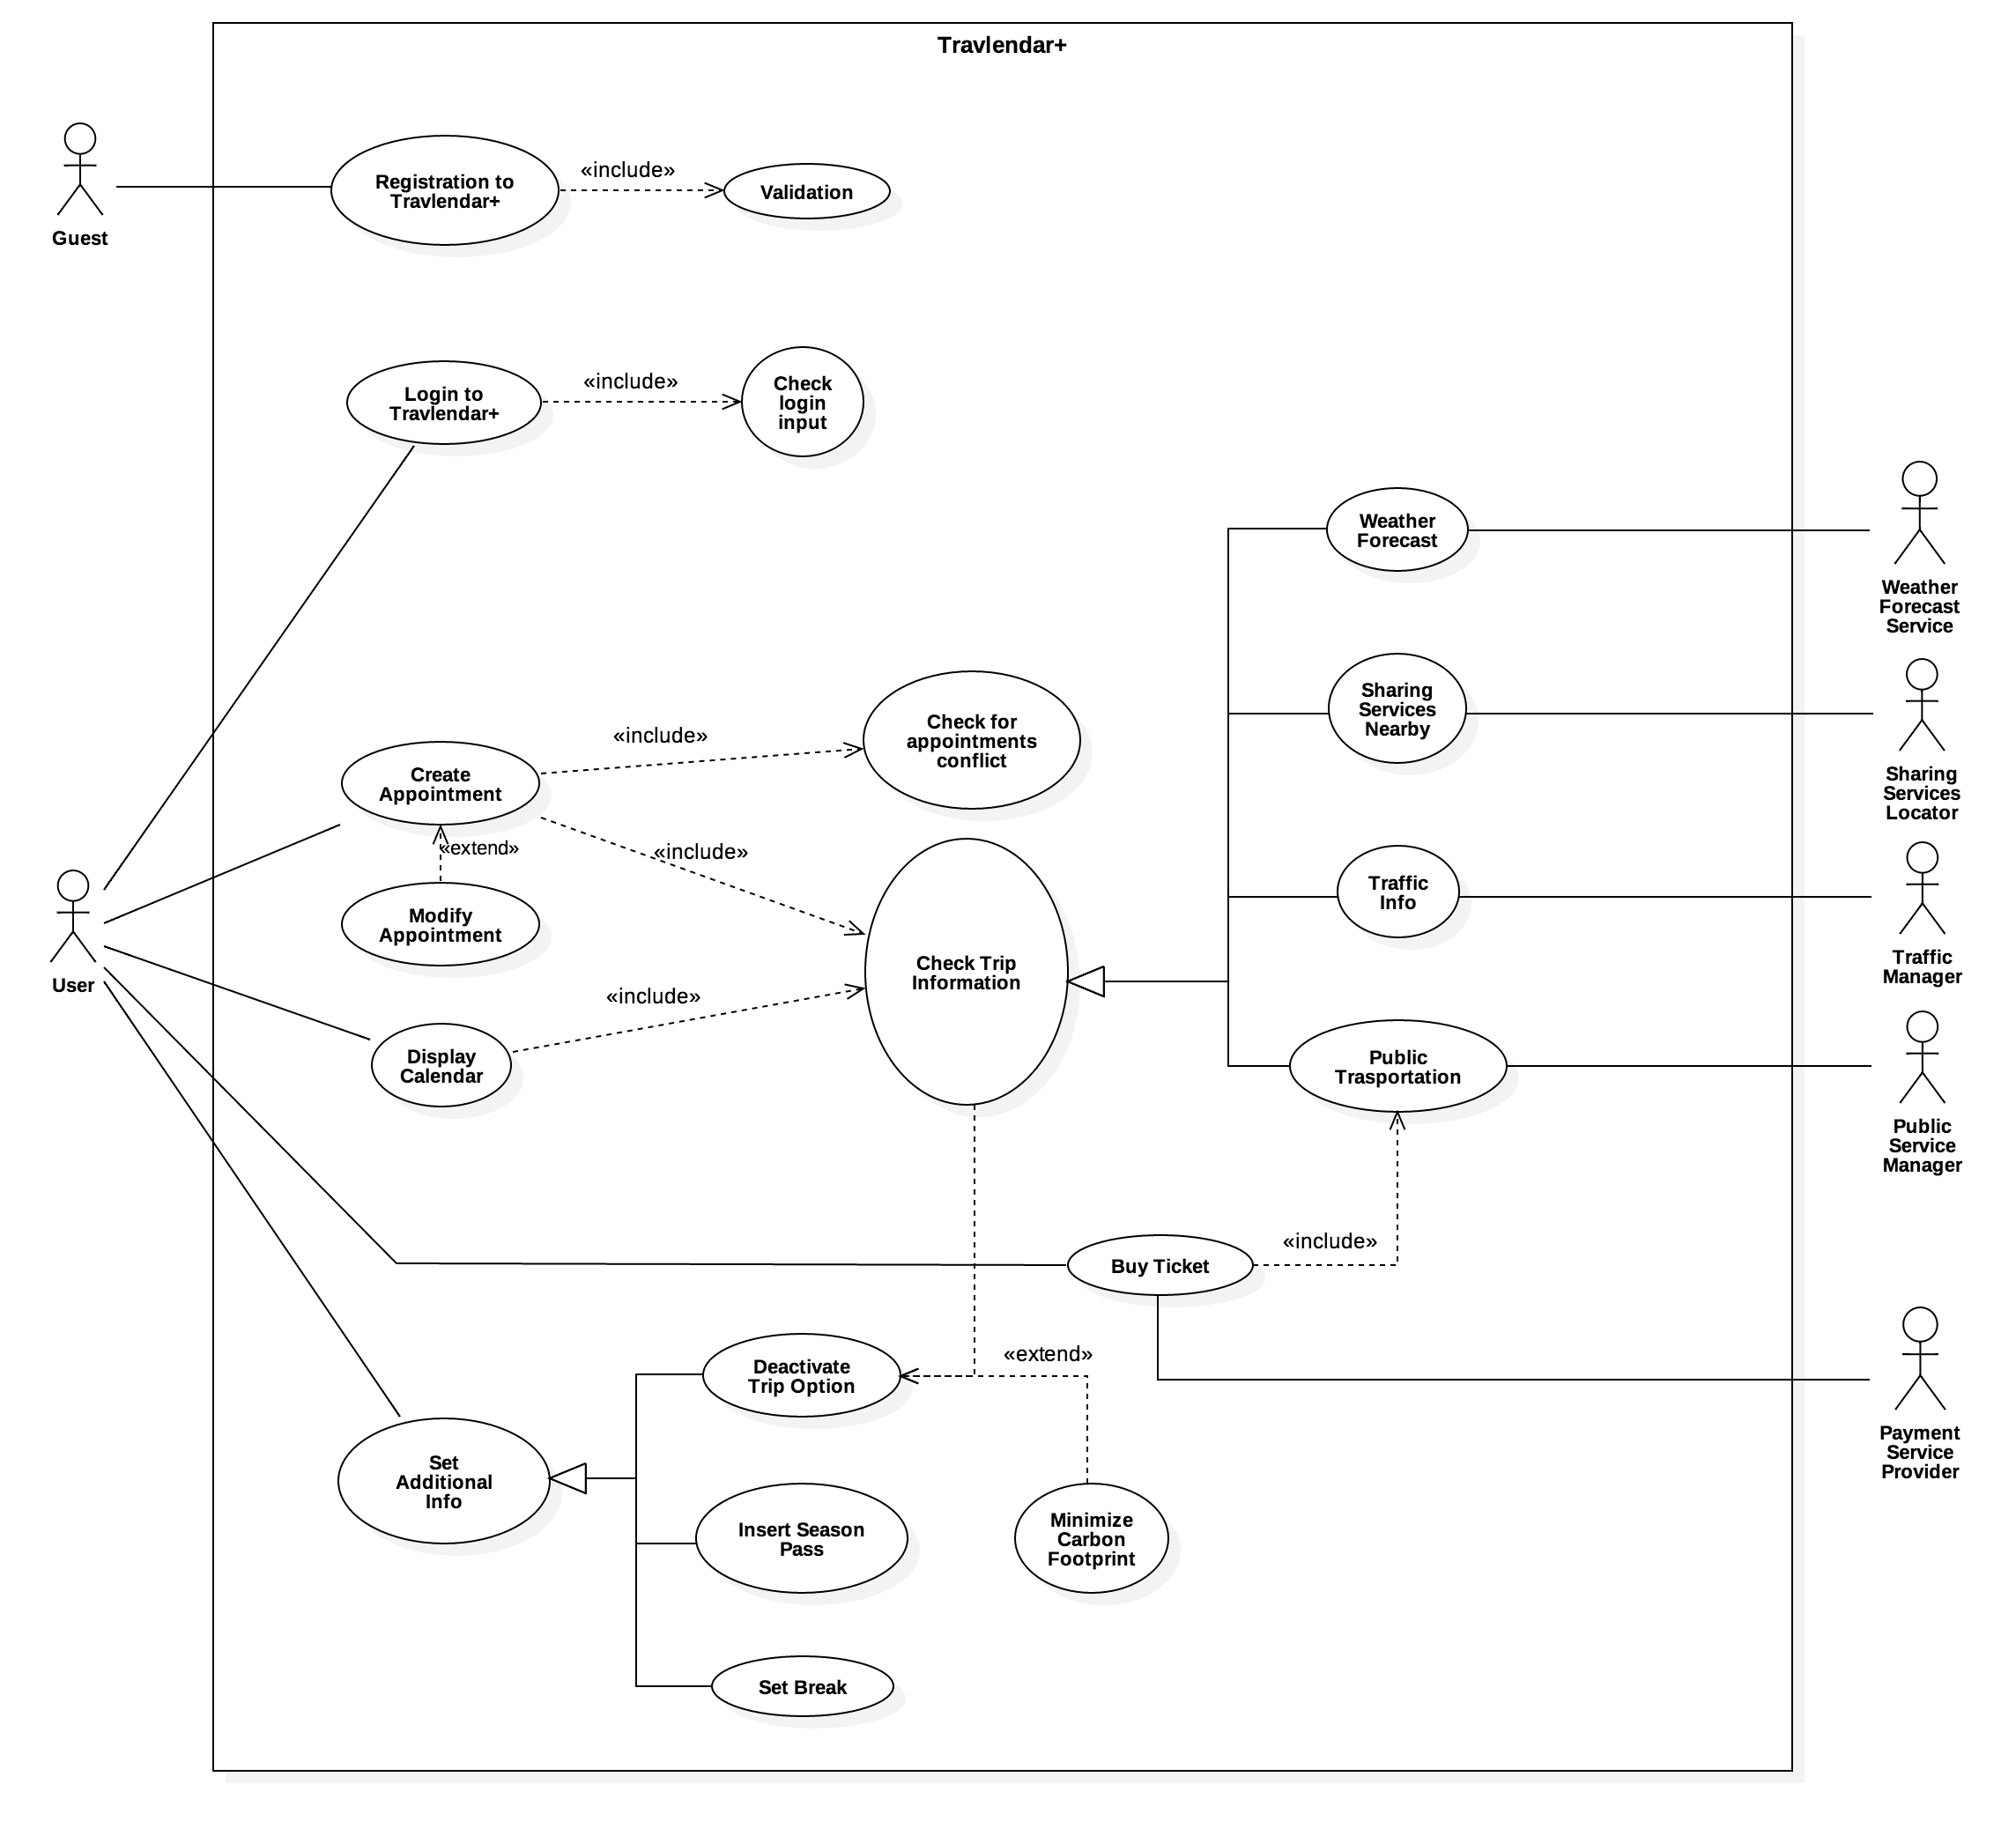
\includegraphics[width=\textwidth]{img/uml/useCase.png}

%%% CREATE A NEW EVENT %%%	
	\paragraph{Use Case 1: Create a New Event}
	
		\begin{tabular}{| l | p{0.8\textwidth} | }
			\hline
			\hline
			Actor	&		User. \\
			\hline
			Input Condition		&		User is already logged in into \textit{Travlendar+}. \\
			\hline
			Event Flow		&		\begin{enumerate}
												\item User click on "\textit{create event}".
												\item User set day, time, place, and event type.
												\item System checks if the new event overlap with already existing events or lunch period.
												\item	 System calculate, ranks and shows multiple solution depending on user travelling preferences.
												\item User select one solution as preferend one.
											\end{enumerate} \\
			\hline
			Output Condition		&		\textit{Tralvendar+} shows calendar main page with the new event. \\
			\hline		
			Exception		&		\begin{itemize}
											\item[-] Created event overlaps with already existing events.
											\item[-] There are no feasible solution.
										\end{itemize} \\
			\hline
			\hline
		\end{tabular}


%%% MODIFY EVENT %%%

	\paragraph{Use Case 2: Modify Event}
	
		\begin{tabular}{| l | p{0.8\textwidth} | }
			\hline
			\hline
			Actor	&		User. \\
			\hline
			Input Condition		&		\begin{itemize}
													\item[-] User is already logged in into \textit{Travlendar+}.
													\item[-] Event Already Exists.
												\end{itemize} \\
			\hline
			Event Flow		&		\begin{enumerate}
												\item User click on "\textit{Event}".
												\item User starts modifying process.
												\item System checks if the new event overlap with already existing events or lunch period.
												\item	 System calculate, ranks and shows multiple solution depending on user travelling preferences.
												\item User select one solution as preferend one.
											\end{enumerate} \\
			\hline
			Output Condition		&		\textit{Tralvendar+} shows calendar main page, with the updated event. \\
			\hline		
			Exception		&		\begin{itemize}
											\item[-] Created event overlaps with already existing events.
											\item[-] There are no feasible solution.
										\end{itemize} \\
			\hline
			\hline
		\end{tabular}
		
		
%%% INSERT PAYMENT METHOD%%%

	\paragraph{Use Case 3: Insert Payment Method}
	
		\begin{tabular}{| l | p{0.8\textwidth} | }
			\hline
			\hline
			Actor	&		User. \\
			\hline
			Input Condition		&		\begin{itemize}
													\item[-] User is already logged in into \textit{Travlendar+}.
													\item[-] Credit Card isn't already inserted on the system.
												\end{itemize} \\
			\hline
			Event Flow		&		\begin{enumerate}
												\item User click on "\textit{Preferences}" and then on "\textit{Payment Methods}".
												\item User sets all the credit cards info.
												\item System checks and validate provided informations.
											\end{enumerate} \\
			\hline
			Output Condition		&		\textit{Tralvendar+} returns to \textit{Payment Methods} page showing added card as a valid payment method. \\
			\hline		
			Exception		&		Credit card given informations are invalid. \\
			\hline
			\hline
		\end{tabular}

%%% BUY TICKET %%%

	\paragraph{Use Case 4: Buy Public Transportation Ticket}
	
		\begin{tabular}{| l | p{0.8\textwidth} | }
			\hline
			\hline
			Actor	&		User. \\
			\hline
			Input Condition		&		\begin{itemize}
													\item[-] User is already logged in into \textit{Travlendar+}.
													\item[-] A \textit{payment method} is already available.
												\end{itemize} \\
			\hline
			Event Flow		&		\begin{enumerate}
												\item User click on "\textit{Buy Ticket}".
												\item System shows available public trasportation services.
												\item User selects a ticket.
												\item	 System starts perchause transaction.
											\end{enumerate} \\
			\hline
			Output Condition		&		Based on public transportation service, User receives a valid ticket. \\
			\hline		
			Exception		&		Transaction doesn't work. \\
			\hline
			\hline
		\end{tabular}


% \input{Subsections/uml/class_diagram.tex}

% \input{Subsections/uml/sequence_diagram.tex}

	\newpage
	\section{Alloy modeling}
	%\subsection{The Model}
	The following model concerns the most characterizing features of the system. We avoided to burden the model with trivial and non-significant details.
	
	\subsubsection*{Data Types}
		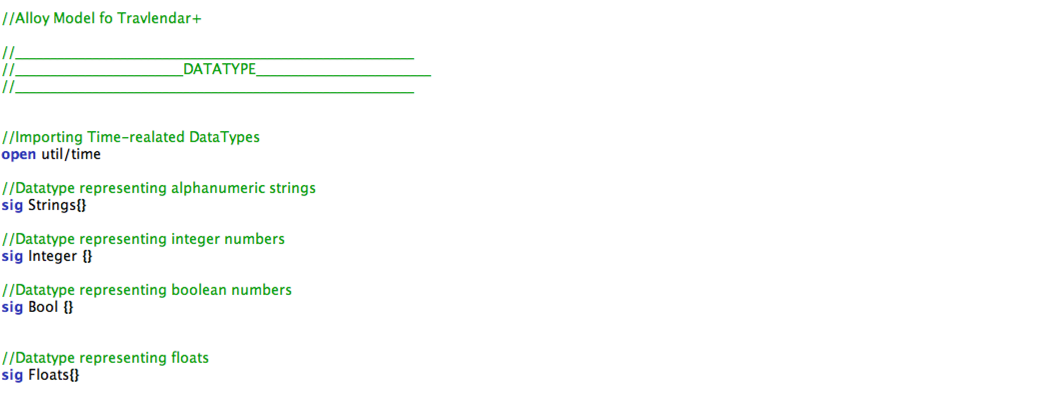
\includegraphics[width = \textwidth]{alloy/code/dataType}

	\subsubsection*{Signatures}
		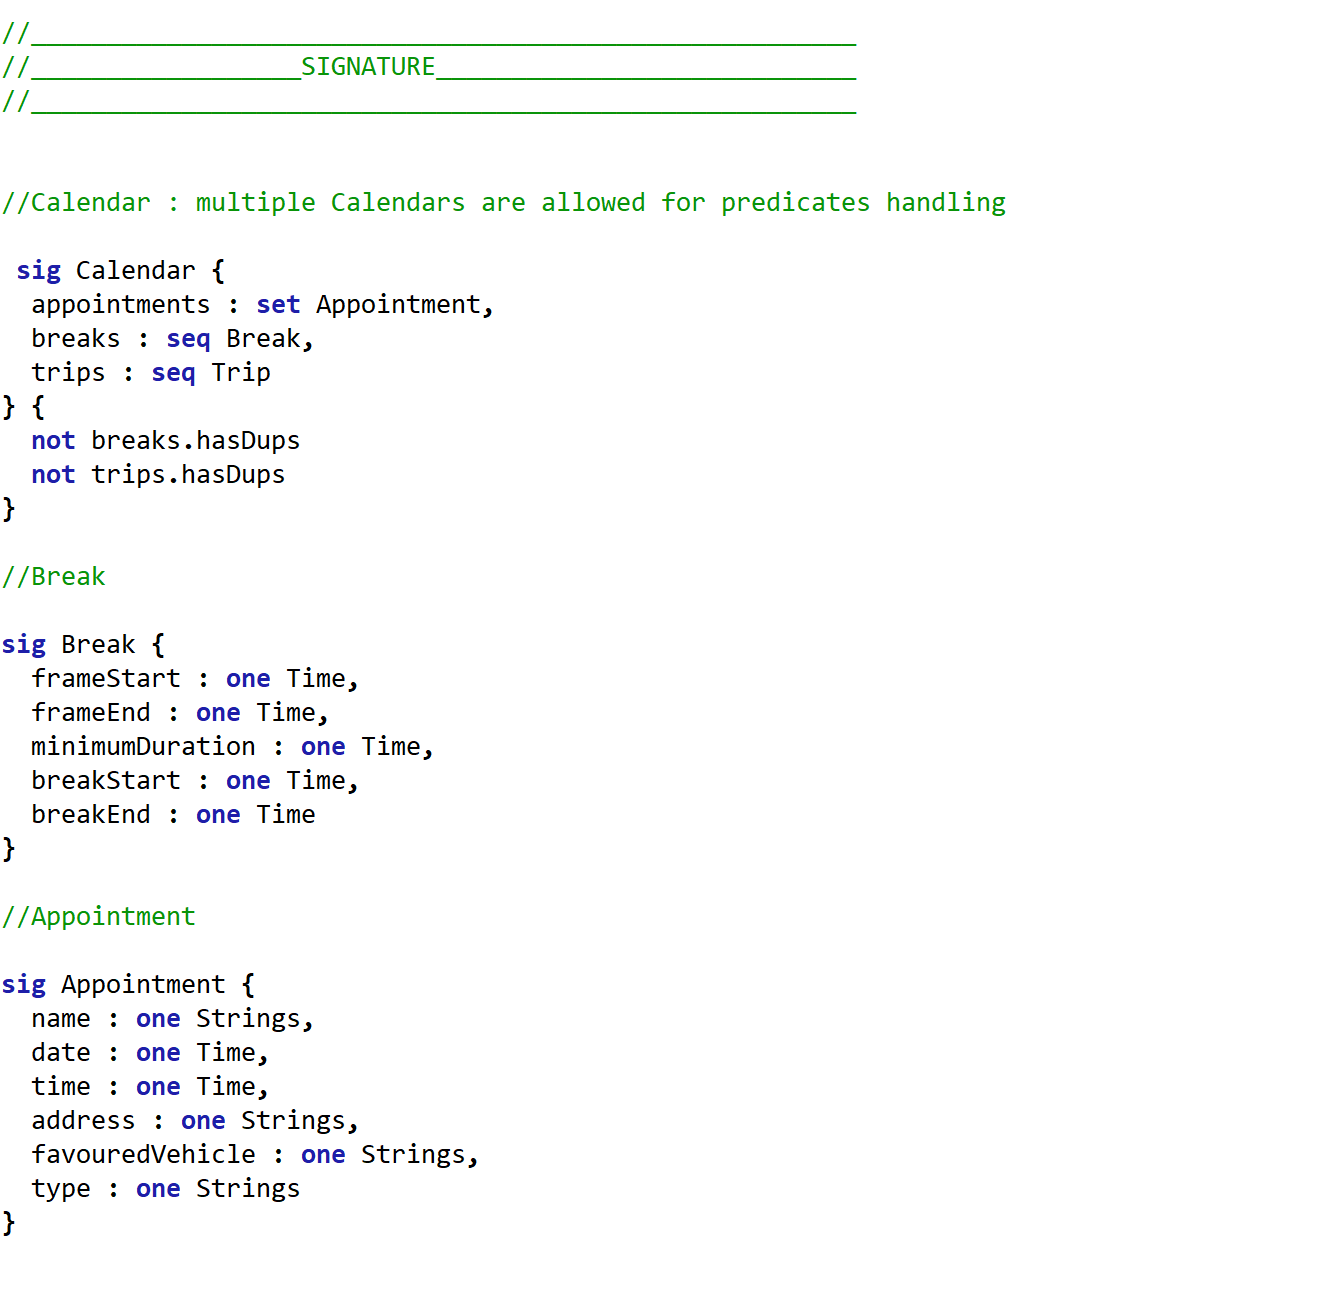
\includegraphics[width = \textwidth]{alloy/code/signature1}
		\vfill
		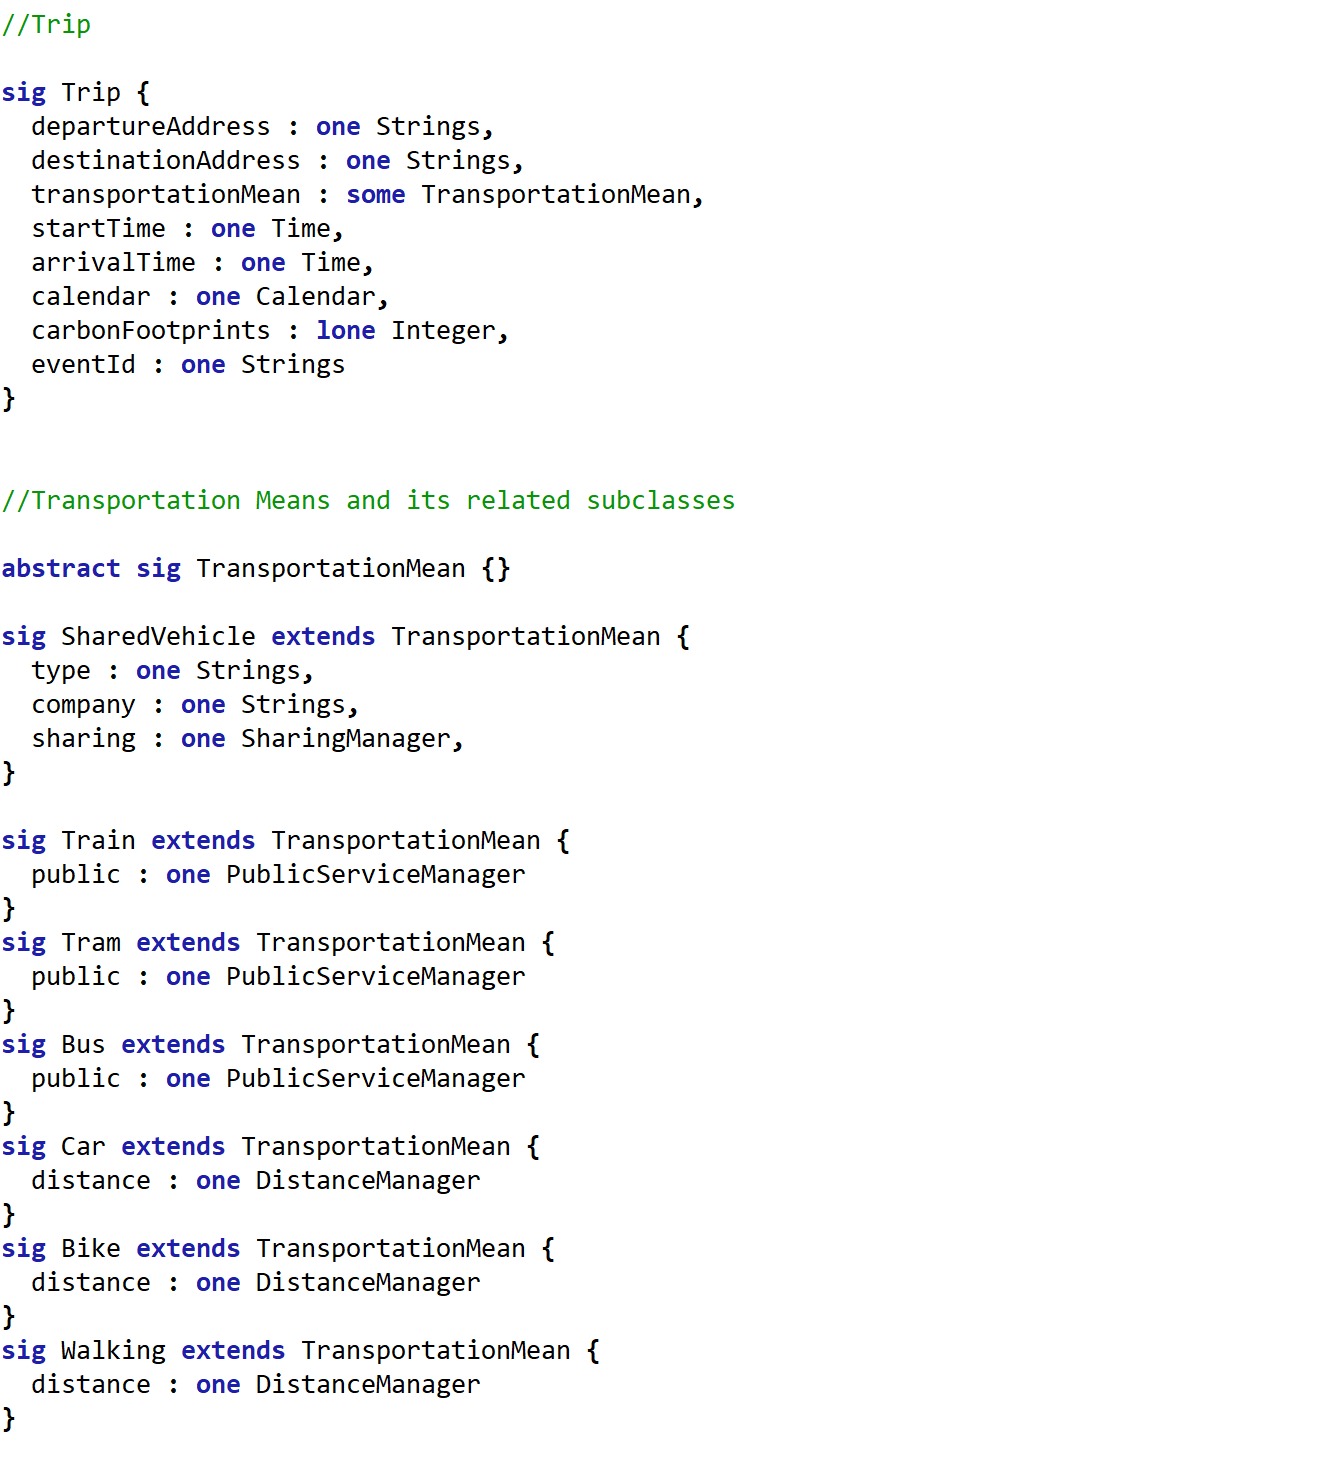
\includegraphics[width = \textwidth]{alloy/code/signature2}
	
	\subsubsection*{Facts}
		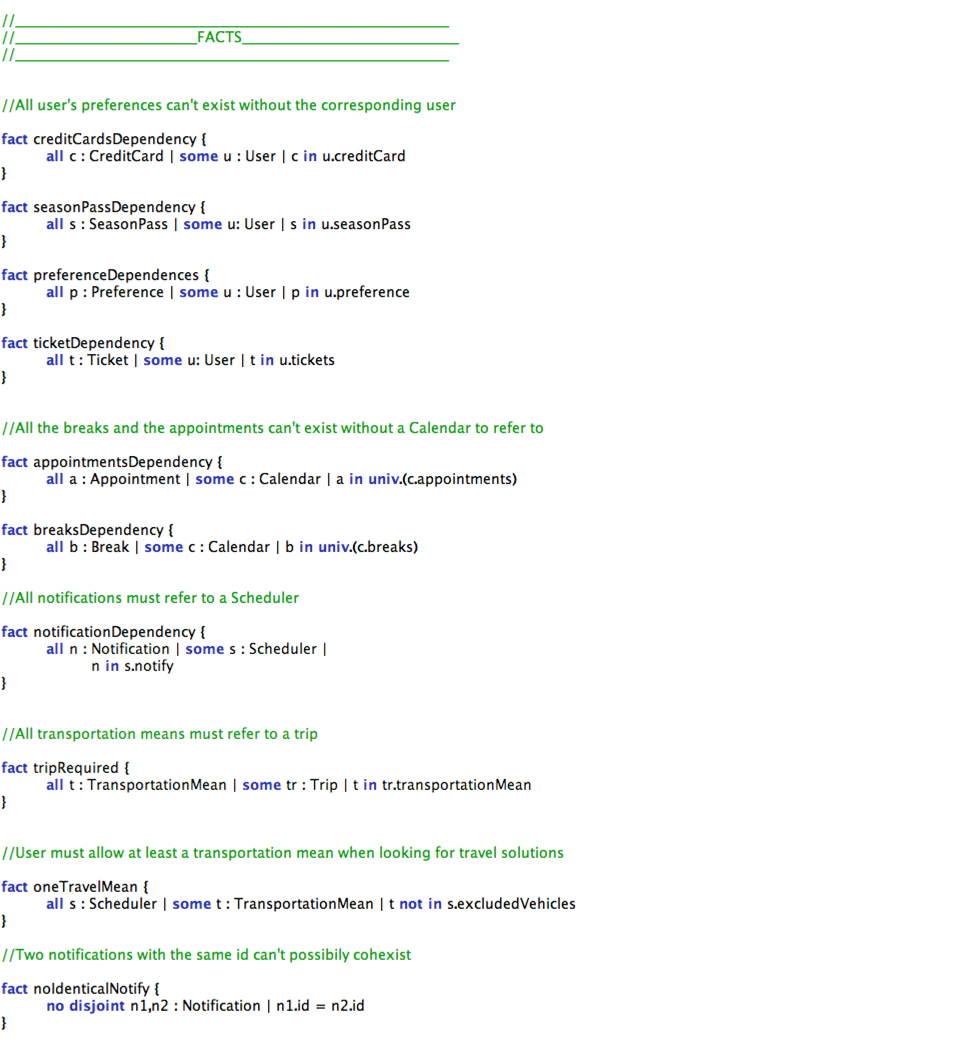
\includegraphics[width = \textwidth]{alloy/code/fact1}
		\vfill
		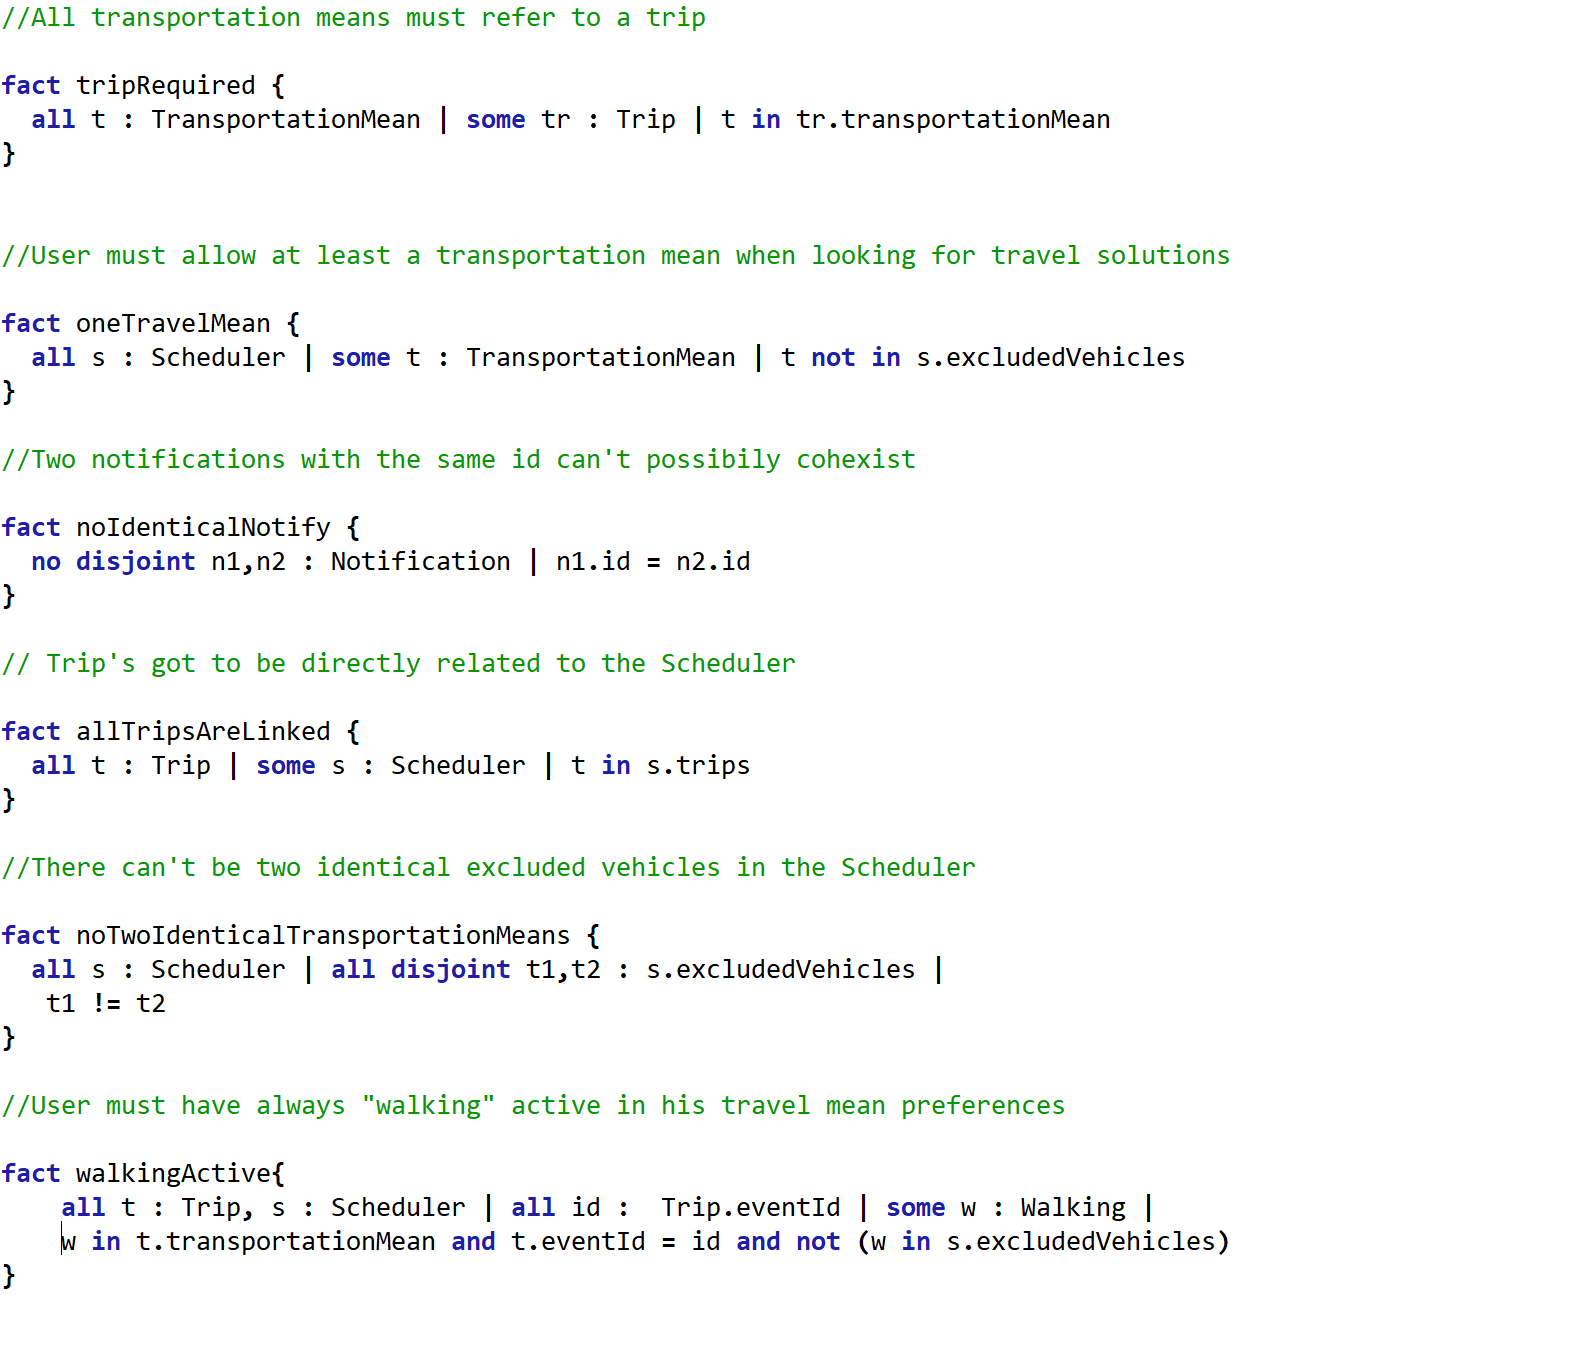
\includegraphics[width = \textwidth]{alloy/code/fact2}
	
	\subsubsection*{Predicates}
		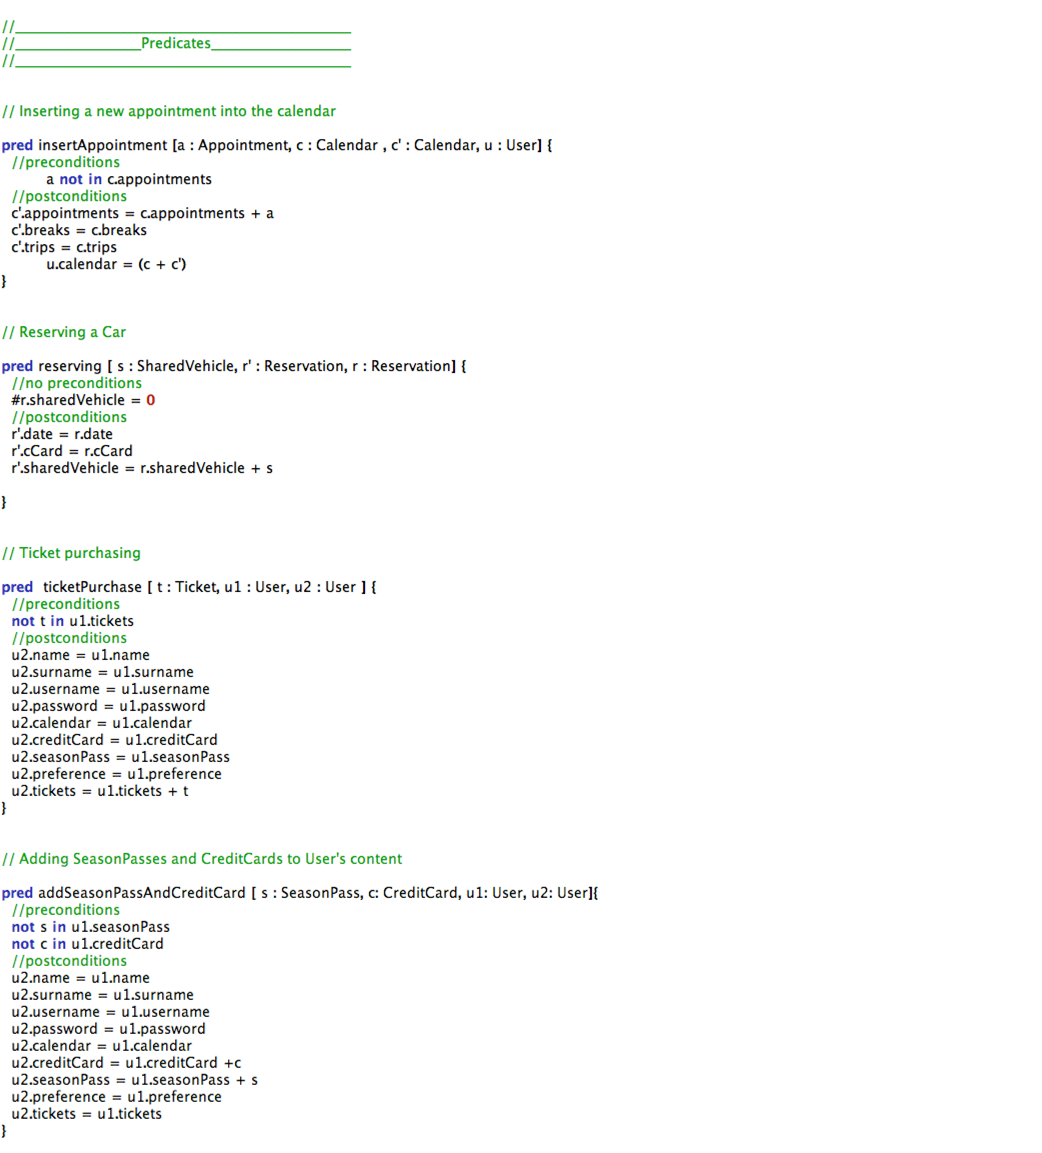
\includegraphics[width = \textwidth]{alloy/code/predicate}
		\bigskip
		
\subsection{Results}
	\begin{figure}[H]
		\centering
		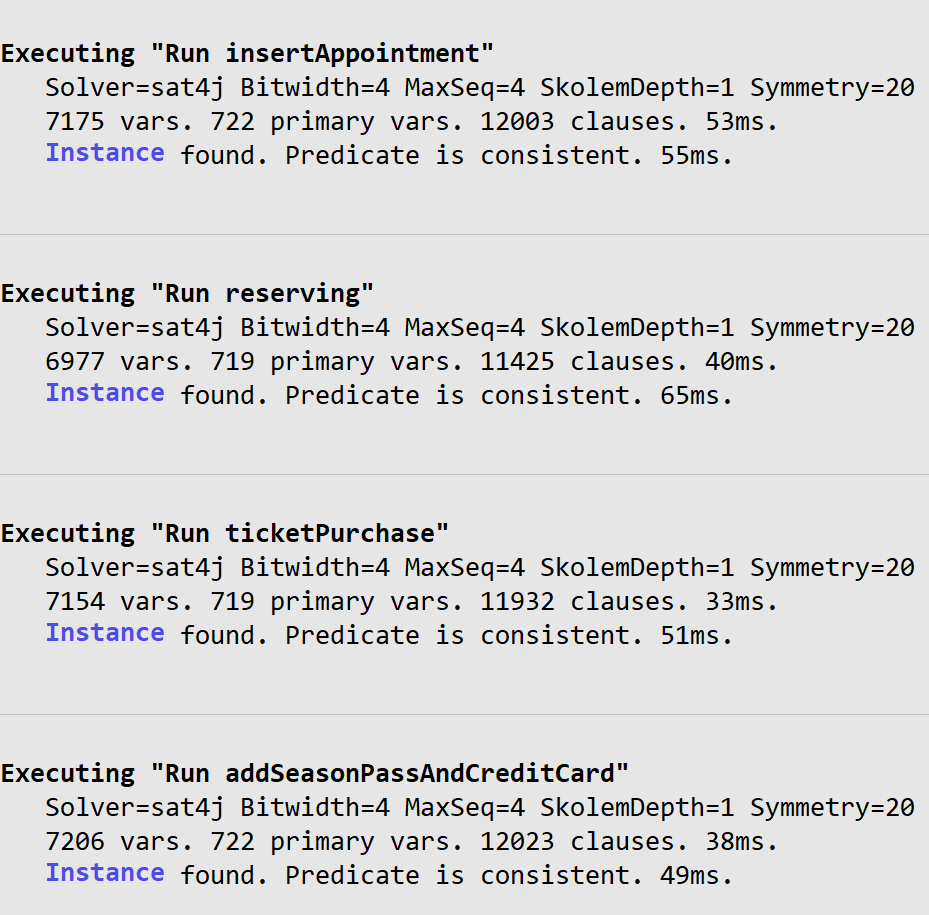
\includegraphics[width = 0.7\linewidth]{alloy/generatedWorld/Results}
		\caption{Result of the model analysis.}		
		\label{fig:alloyResult}
	\end{figure}
	\bigskip
	
	
	
	

\begin{landscape}
	\subsection{Generated World}
	
		\subsubsection{World Generated}
			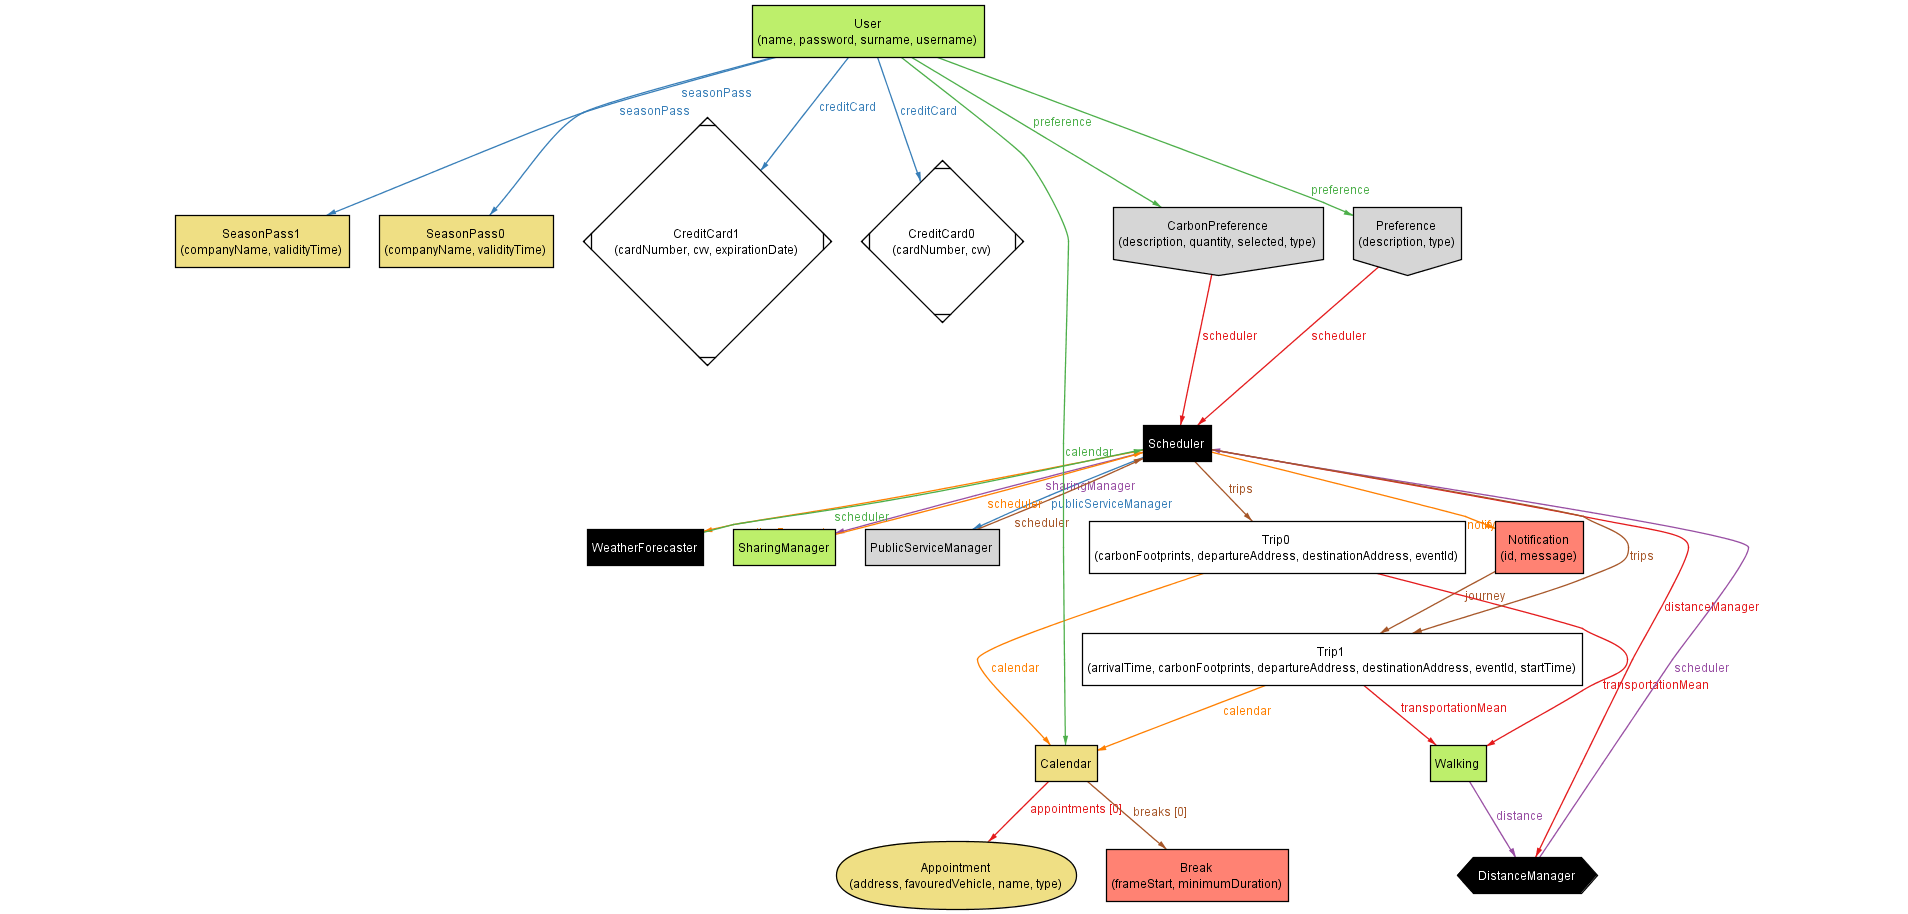
\includegraphics[height= 0.9\textheight , center]{alloy/generatedWorld/WorldGenerated}
	
		\subsubsection{Ticket Purchase}
			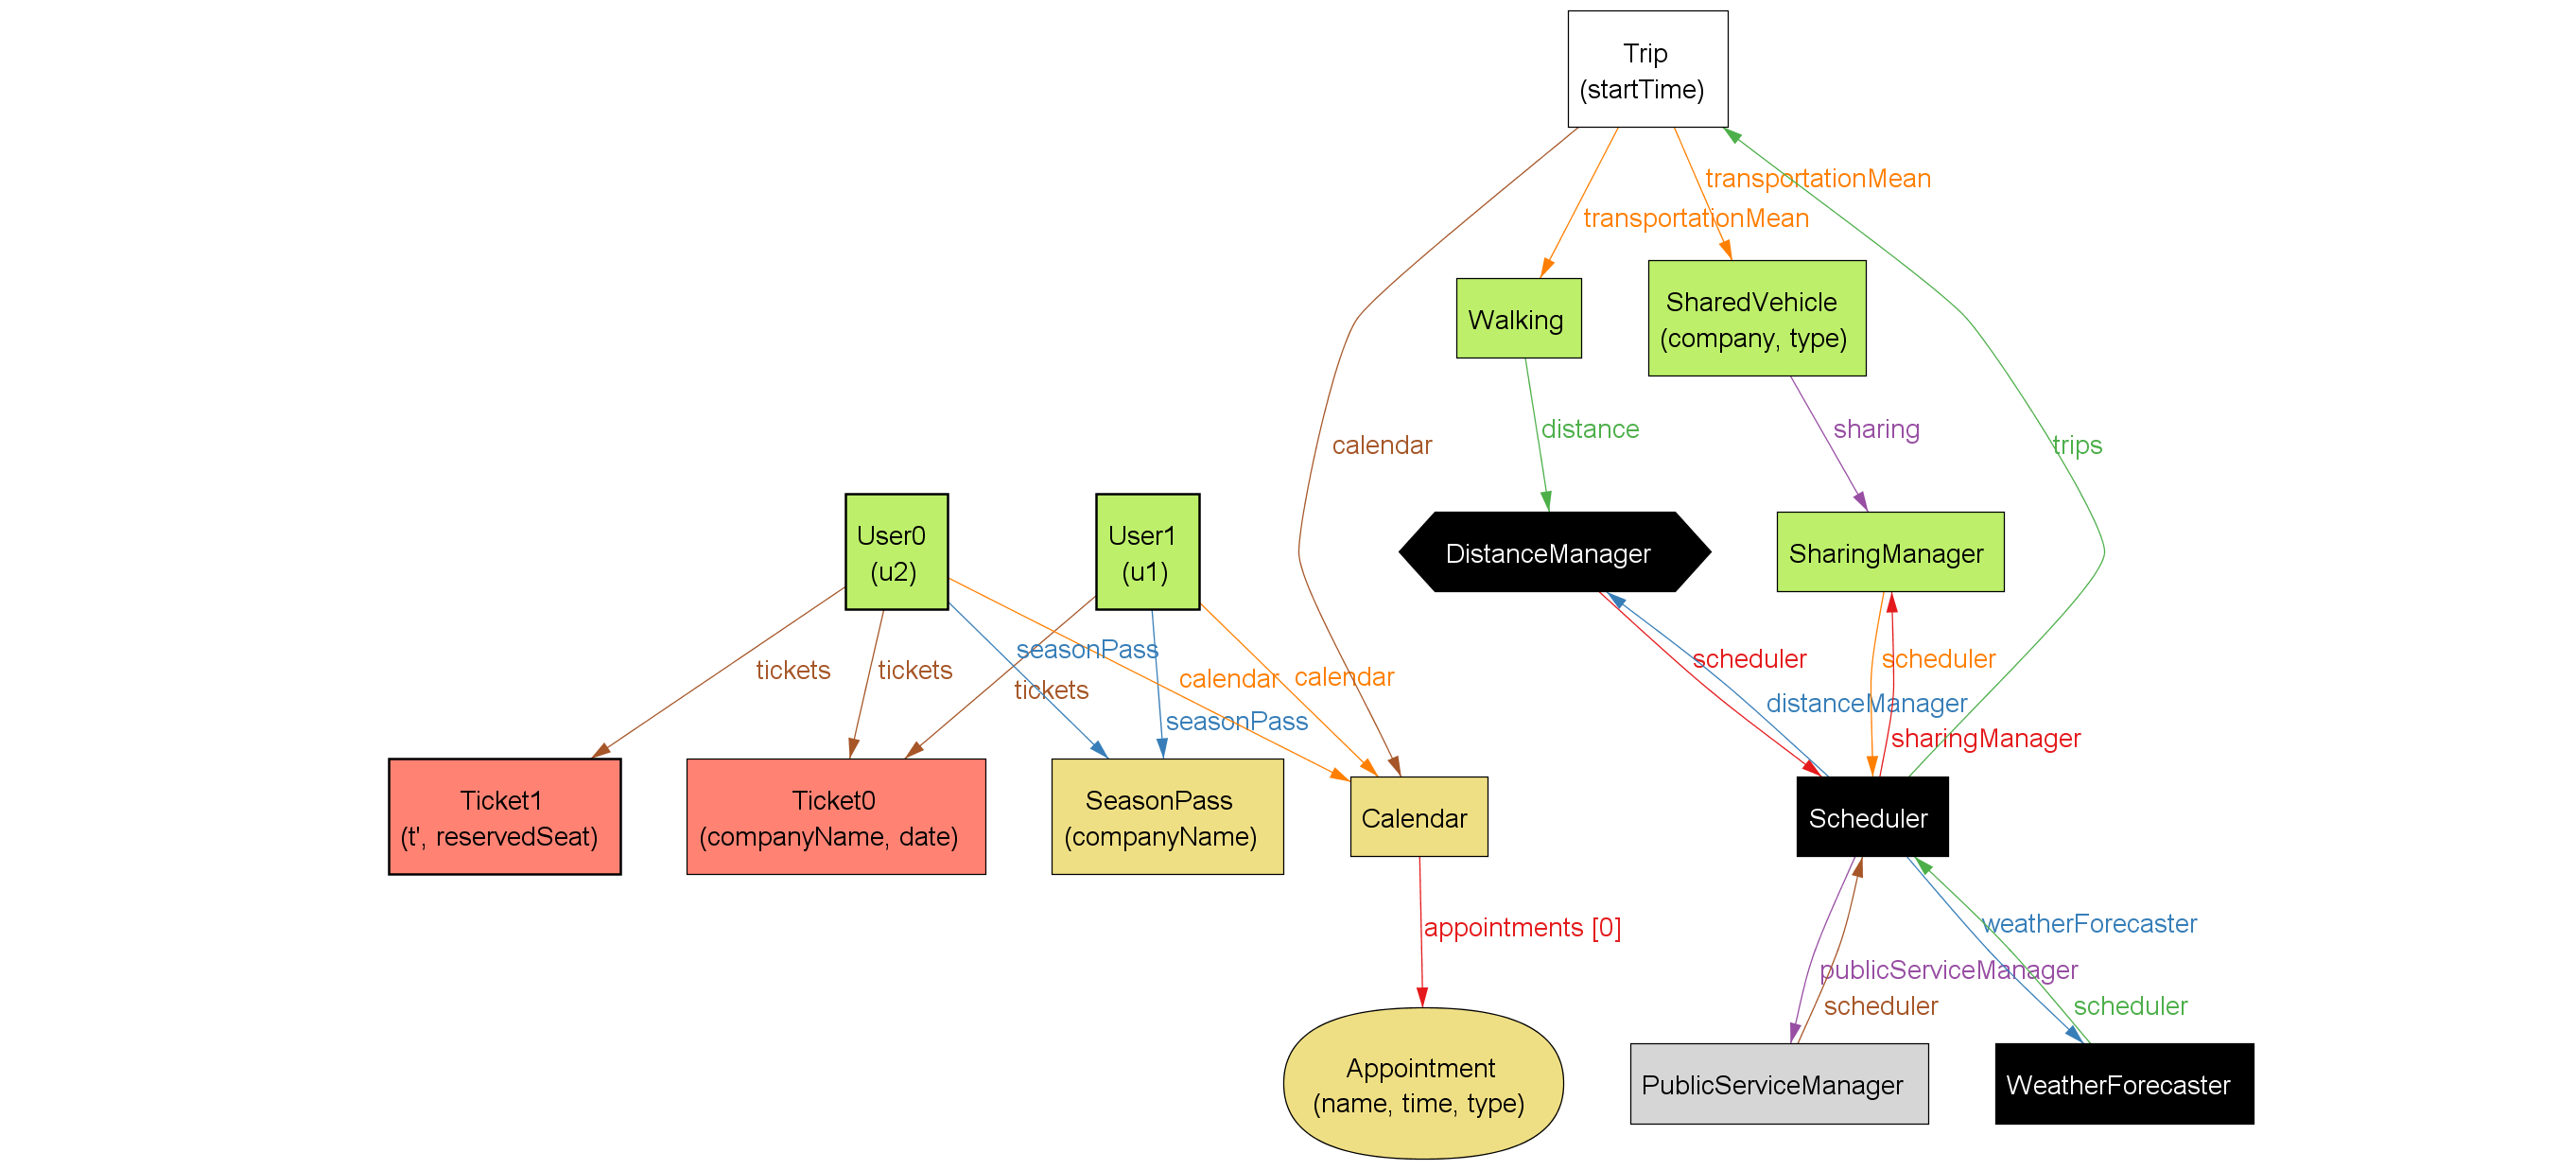
\includegraphics[height= 0.9\textheight, width= 35cm, center]{alloy/generatedWorld/ticketPurchase}
	
		\subsubsection{Renting}
			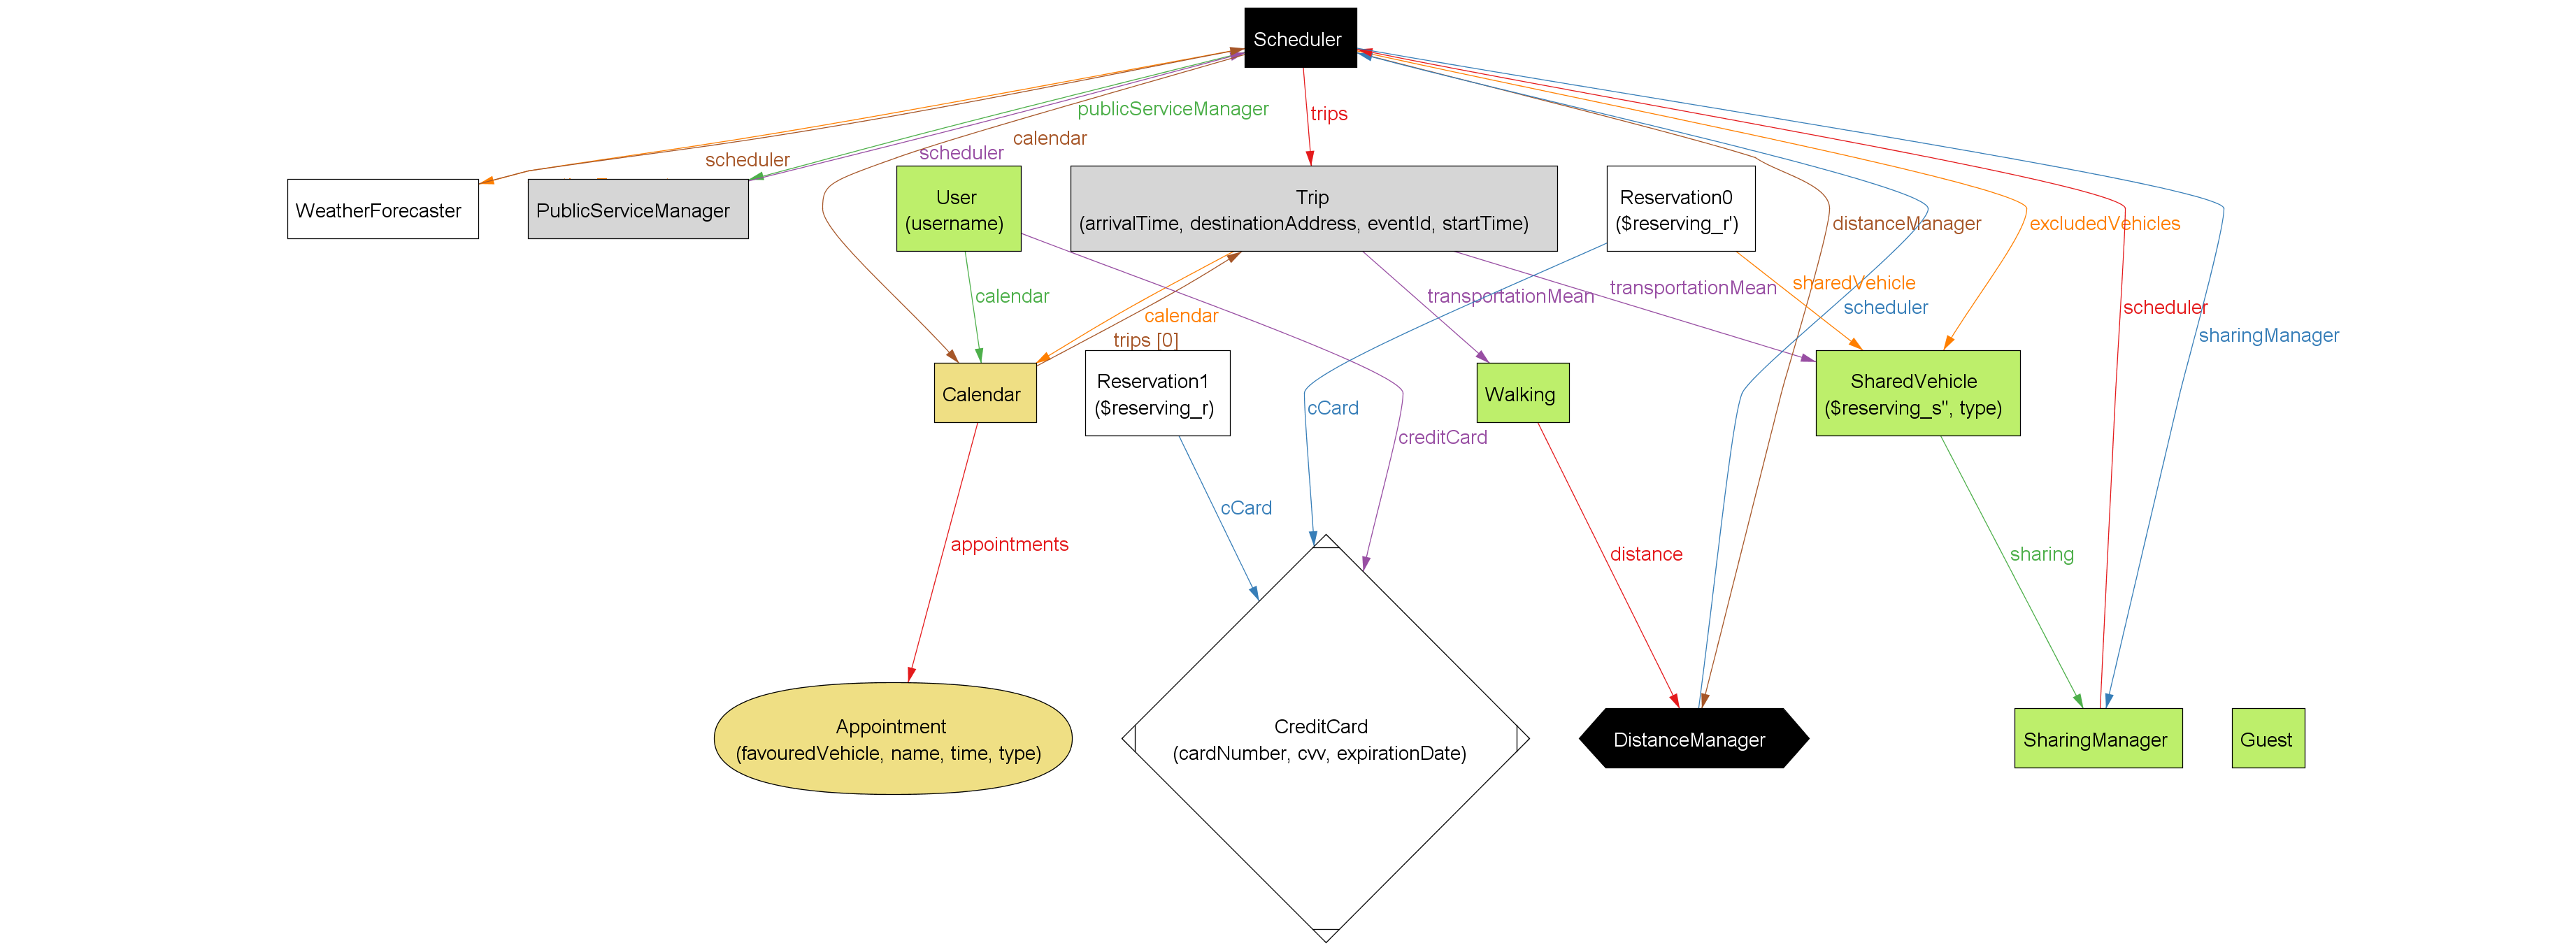
\includegraphics[height = 0.9\textheight, width= 35cm, center]{alloy/generatedWorld/reserving}
		
		\subsubsection{Insert Appointment}
			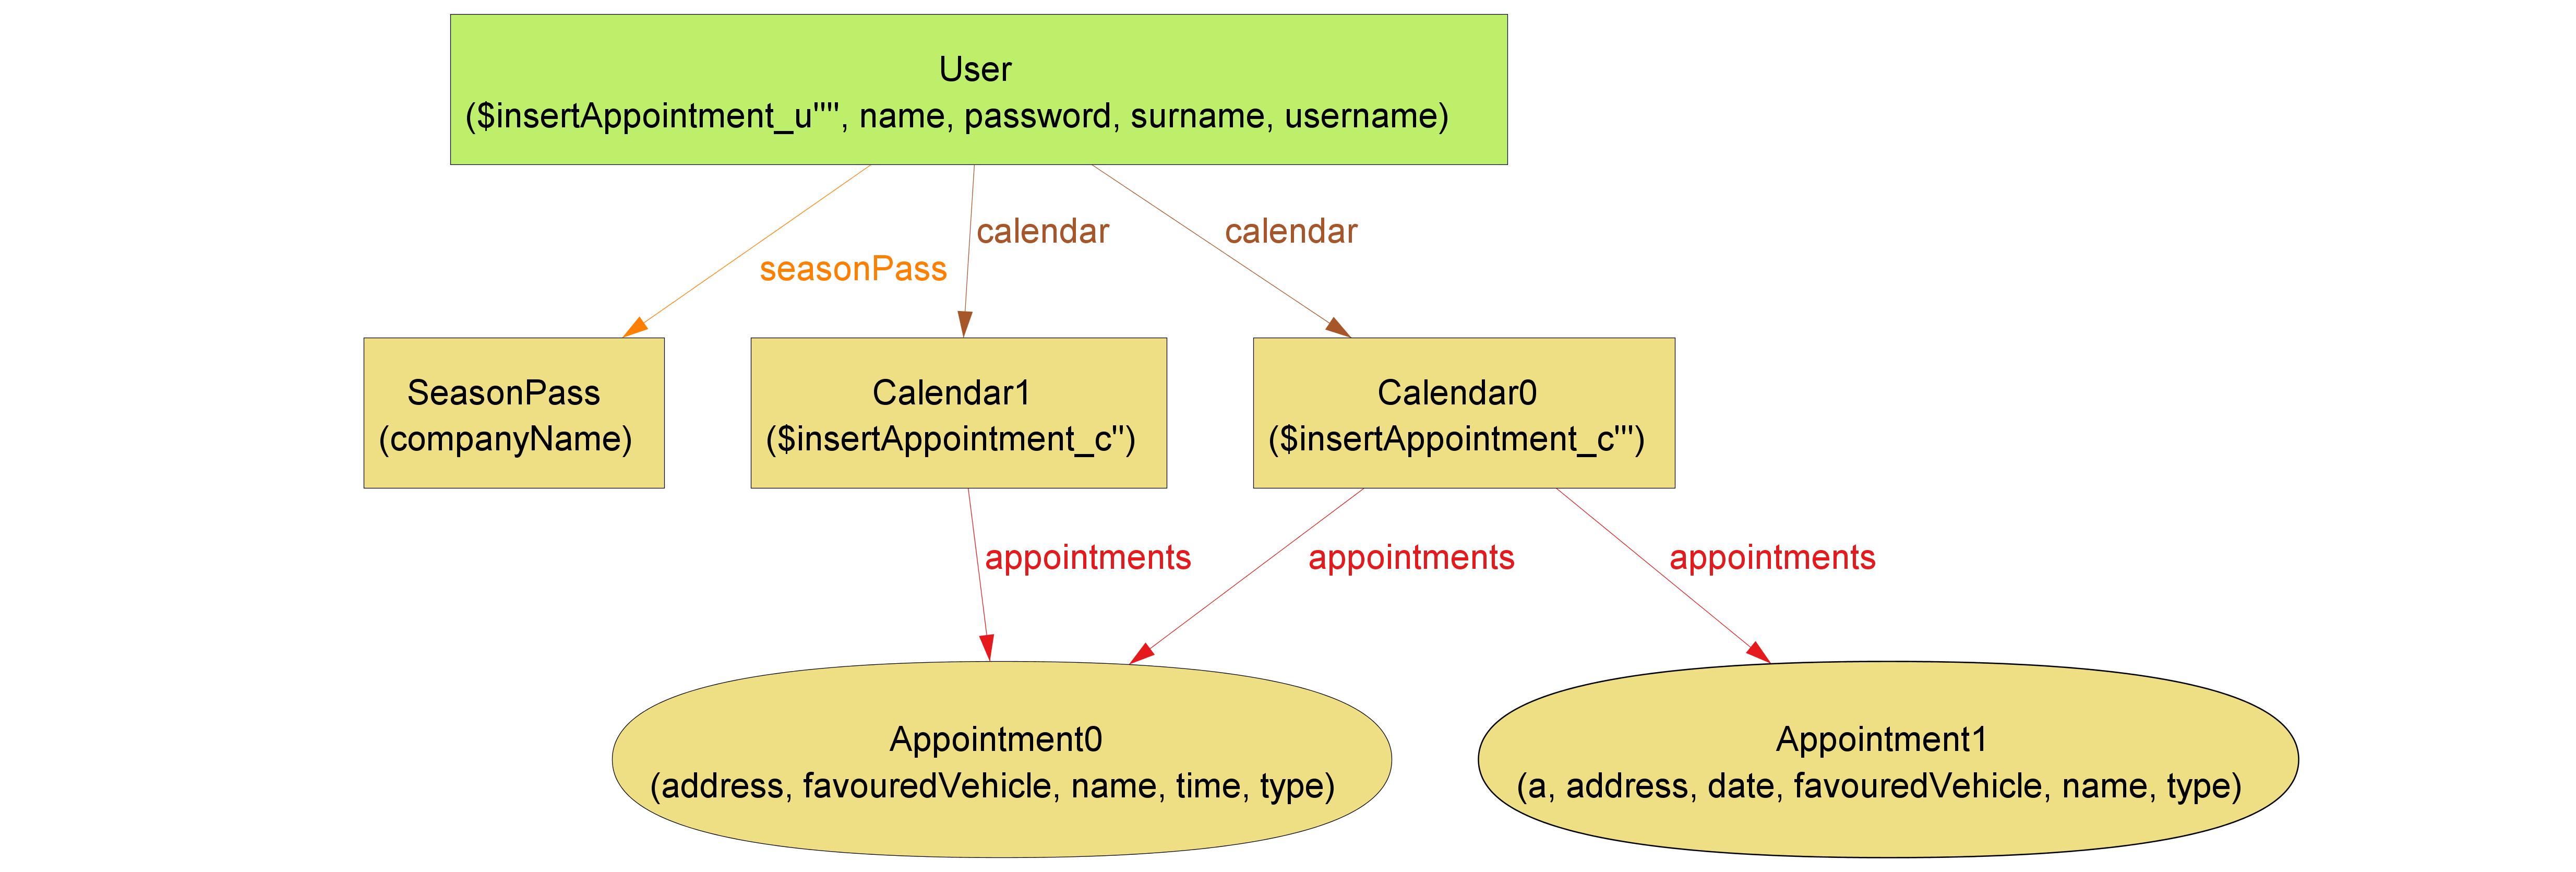
\includegraphics[height = 0.7\textheight, width= 25cm, center]{alloy/generatedWorld/insertAppointment}
			
		\subsubsection{Add SeasonPass and Credit Card}
			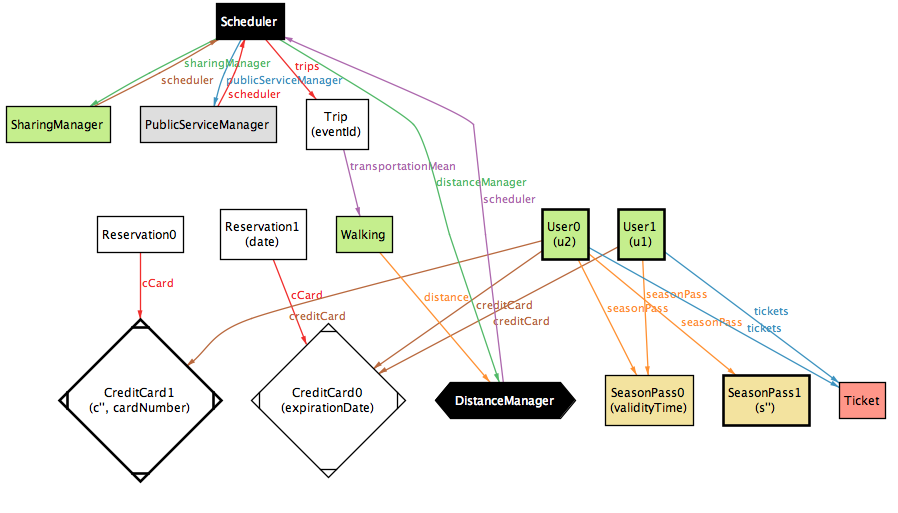
\includegraphics[height = 0.7\textheight, width= 25cm, center]{alloy/generatedWorld/addSeasonPassAndCreditCard}

\end{landscape}
	
	


	\newpage
	%%% appendix %%%
	\section{Appendix}
		\listoffigures
		\listoftables
		
		\subsection{Used tools}
		For this assignment, we used the following tools:
		
		\begin{description}
			\item [Alloy] We used the alloy tool to write the code and check the models for the specification.
			\item [LaTeX] The group used LaTeX to structure the final document and to help with versioning.
			\item [Github] We leaned on Github for versioning and coordinating synchronized work.
			\item [Toggl] We used toggl to keep track of work hours.
			
		\end{description}
		
		\subsection{Hours of work}
			\begin{description}
				\item[Bisica, Leonardo] around xx hours of work;
				\item[Castellani, Alessandro] around xx hours of work;
				\item[Cataldo, Michele] around xx hours of work.
			\end{description}
			
\end{document}